\chapter{Многоспиновая запутанность в системе эквивалентных спинов}
\label{chapter:manyparticle-entanglement-in-nanopore}
% \subsection{Создание дипольно упорядоченных состояний}
% (PRA-2019)
%   - Температурная зависимость многочастичной запутанности
%   - Зависимость от числа частиц
%
% Многоспиновая запутанность c дипольно упорядоченном начальном

% JETP-2020


Результат полученный в предыдущей главе~\ref{chapter:quantum-fisher-information-measurement}
позволяет в рамках МК динамики ЯМР прояснить более глубокие связи между MK когерентностями ЯМР и запутанностью.
Эти связи соответствуют распространению МК корреляций внутри многочастичной системы в процессе эволюции.
В результате из второго момента спектра интенсивности МК когерентностей ЯМР
можно извлечь информацию о многочастичной запутанности и свидетелях запутанности.

Для исследования многочастичной запутанности необходимо работать с моделью,
которая содержит достаточно большое ($>50$) количество взаимодействующих спинов,
и может быть экспериментально исследована при низких температурах.
Только тогда можно будет исследовать многочастичную запутанность и ее зависимость от температуры.
В разделе~\ref{sec:model-equivalent-spins} была рассмотрена несферическая нанопора,
заполненная газом со спин-несущими атомами (например, ксеноном) или молекулами в сильном внешнем магнитном поле.
Эта модель полностью отвечает поставленным требованиям.
По существу нанопора является системой эквивалентных спинов,
и ее МК динамика ЯМР может быть исследована точно.

На подготовительном периоде МК эксперимента ЯМР гамильтониан системы эквивалентных спинов
определяется выражением (см~\ref{sec:model-equivalent-spins})
\begin{equation}\label{eq:mq-hamiltoninan-equivalent-spins}
  H_\mathrm{MQ} = - \dfrac{D}{4} \left[
    \left( I^{+} \right)^2 + \left( I^{-} \right)^2
  \right],
  \quad
  I^{\pm} = \sum\limits_{j=1}^{N} I^{\pm}_j,
\end{equation}
где $I^{\pm}_{j}$ --- повышающий или понижающий операторы спина $j$,
$N$ --- число спинов в нанопоре,
$D$ - константа диполь-дипольного взаимодействия (ДДВ),
усредненная по быстрой молекулярной диффузии спин-несущих атомов (молекул) в нанопоре.
Как уже было обсуждено в разделе~\ref{sec:model-equivalent-spins},
гамильтониан $H_\mathrm{MQ}$
коммутирует с квадратом полного спинового углового момента $\hat I^2$,
поэтому удобно перейти к базису,
состоящего из общих собственных состояний $\hat I^2$ и $I_z$.
В этом базисе гамильтониан $H_{MQ}$ состоит из блоков $H_{MQ}^S$, соответствующих различным значениям полного спинового углового момента $S$:
\begin{equation}
  \hat I^2 = S(S+1), S = N/2, N/2-1, N/2-2,
\end{equation}
где
$N/2 - [N/2]$, $[i]$ - целая часть $i$.

Далее в этой главе будут рассмотрены два наиболее интересных начальных состояний системы
и исследованы температурные зависимости многоспиновой запутанности для каждого случая.

\section{Термодинамически равновесное начальное состояние}
\label{sec:nanopora-thermodynamic-equilibrium}

Для исследования многочастичной запутанности в зависимости от температуры,
в этом разделе будет рассмотрена МК динамика ЯМР
системы эквивалентных спинов размера $N$
с начальным термодинамически равновесным состоянием $\rho_\mathrm{eq}$:
%
\begin{equation}\label{eq:rho_eq}
  \rho(0) = \rho_{\mathrm{eq}} = \dfrac{e^{\frac{\hbar\omega_{0}}{kT} I_z}}{Z},
\end{equation}
%
где $Z =\mathrm{Tr}\left\{e^{\frac{\hbar\omega_{0}}{kT} I_z}\right\}$ это статистическая сумма,
$\hbar$ и $k$ --- это постоянная Планка и постоянная Больцмана,
$\omega_0$ --- Ларморовская частота,
$T$ --- температура,
и $I_z$ это оператор проекции полного углового момента на ось $z$,
которая направлена вдоль сильного внешнего магнитного поля.
%
Существующий теоретический подход~\cite{Doronin2009, Doronin2011}
к МК динамике ЯМР системы эквивалентных спинов
применим только в высокотемпературной области.
Для исследования многочастичной запутанности,
необходимо разработать теорию МК динамики ЯМР системы эквивалентных спинов
для произвольных температур,
что будет сделано ниже.
% Так же будут приведены вычисления для системы из 51, 75, 101, 201 спинов,
% но, в принципе, аналогичные расчеты можно провести и для систем с несколькими тысячами спинов.

Поскольку и гамильтониан $H_{MQ}$, и матрица начальной плотности из уравнения~(\ref{eq:rho_eq}) имеют блочную структуру,
можно заключить,
что эволюционная матрица плотности $\rho_\mathrm{LT}(\tau)$:
%
\begin{equation}
  \label{eq:rho_eval_lt}
  \rho_\mathrm{LT} (\tau) = e^{-iH_\mathrm{MQ}\tau} \rho_\mathrm{eq} e^{iH_\mathrm{MQ}\tau},
\end{equation}
%
также состоит из блоков $\rho^S_\mathrm{LT}(\tau)$,
где $(S=\frac N 2, \frac N 2 - 1, \dots, \frac N 2 - \left[\frac N 2\right])$.
Введем обозначение $\rho^S_{\mathrm{LT}, n}(\tau)$ для
вклада в $\rho^S_\mathrm{LT}(\tau)$ от МК когерентности ЯМР порядка $n$.
Тогда вклад $J_{\mathrm{LT}, n, S}(\tau)$ в интенсивность приведенной МК когерентности ЯМР $n$-го порядка определяется как
%
\begin{equation}
    \label{eq:coherence_k_s}
    J_{\mathrm{LT}, n, S}(\tau) = \dfrac{\mathrm{Tr}\left\{
        \rho_{LT, n}^S(\tau)\rho_{LT, -n}^S(\tau)
    \right\}}
    {\mathrm{Tr}\left\{\rho^2_{eq}\right\}}.
\end{equation}
%
Таким образом задача вычисления когерентностей сводится к вычислению отдельных вкладов для каждого значения полного углового момента $S$.

Наблюдаемые интенсивности приведенных МК когерентностей ЯМР рассчитываются по формуле:
%
\begin{equation}\label{eq:coherence_k}
  J_{\mathrm{LT}, n}(\tau) = \sum\limits_S n_N(S) J_{\mathrm{LT}, n, S}(\tau),
  \quad
  (-N\leq n \leq N),
\end{equation}
%
где $n_N(S)$ --- это кратность интенсивности $J_{n, S}(\tau)$,
определенная в разделе~\ref{sec:model-equivalent-spins} в~(\ref{eq:coeff_n}).


\subsection{Аналитическое решение для трехспиновой системы}
\label{sec:sec:nanopora-thermodynamic-equilibrium-exact_sol}

% \begin{figure}[H]
%   \centering
%   \includegraphics{exact_j.pdf}
%   \caption{Intensities of MQ NMR coherences $J_n, \quad n=0, 2$ in a nanopore with $N = 3$.}
%   \label{fig:exact_j}
% \end{figure}

В этом разделе будет рассмотрена система из $N=3$ спинов
связанных $H_{MQ}$ гамильтонианом,
определенном в выражении (\ref{eq:mq-hamiltoninan-equivalent-spins}).
Возможными значениями полного углового момента спина $S$
являются $\frac 3 2$ и $\frac 1 2$.
Ненулевые элементы блока гамильтониана $H_{MQ}^{S}$ определены в выражении~(\ref{eq:i-square-elements}).
Матричное представление $H_{MQ}^{3/2}$ имеет вид
%
\begin{equation}
    \label{eq:ham_3_2}
    H_{MQ}^{3/2} =
    \begin{pmatrix}
        0 & 0 & -\frac{\sqrt{3} D}{2} & 0 \\
        0 & 0 & 0 & -\frac{\sqrt{3} D}{2} \\
        -\frac{\sqrt{3} D}{2} & 0 & 0 & 0 \\
        0 & -\frac{\sqrt{3} D}{2} & 0 & 0
    \end{pmatrix}.
\end{equation}
%
Собственные значения $\lambda_{3/2}^{(i)}(i=1, 2, 3, 4)$
блока гамильтониана $H_{MQ}^{3/2}$ следующие
%
\begin{equation}\label{eq:eigvals_3_2}
  \lambda_{3/2}^{(1)} = -\frac{\sqrt{3} D}{2}, \quad
  \lambda_{3/2}^{(2)} = -\frac{\sqrt{3} D}{2}, \quad
  \lambda_{3/2}^{(3)} = \frac{\sqrt{3} D}{2}, \quad
  \lambda_{3/2}^{(4)} = \frac{\sqrt{3} D}{2}.
\end{equation}
%
Соответствующий набор собственных векторов выглядит следующим образом:
%
\begin{align}\label{eq:eigvecs_3_2}
  u_{3/2}^{(1)} & =  \left(\frac{1}{\sqrt{2}}, 0, \frac{1}{\sqrt{2}}, 0\right) ,
  \notag \\
  u_{3/2}^{(2)} & =  \left(0, \frac{1}{\sqrt{2}}, 0, \frac{1}{\sqrt{2}}\right) ,
  \notag \\
  u_{3/2}^{(3)} & =  \left(-\frac{1}{\sqrt{2}}, 0, \frac{1}{\sqrt{2}}, 0\right) ,
  \notag \\
  u_{3/2}^{(4)} & =  \left(0, -\frac{1}{\sqrt{2}}, 0, \frac{1}{\sqrt{2}}\right) .
\end{align}
%
Блок $H^{1/2}_{MQ}$ является скаляром
%
\begin{equation}\label{eq:ham_1_2}
  H^{1/2}_{MQ} = 0.
\end{equation}
%
Блоки эволюционной матрицы плотности $\rho_\mathrm{LT}^{n/2}(\tau) \quad (n = 1, 3)$
могут быть вычислены по формуле
%
\begin{equation}\label{eq:liouvile_sol}
  \rho_\mathrm{LT}^{n/2}(\tau) =
  U_{n/2} e^{-i\Lambda^{n/2}\tau} U^{+}_{n/2}
  \rho^{n/2}_\mathrm{LT}(0)
  U_{n/2} e^{i\Lambda^{n/2}\tau} U^{+}_{n/2},
\end{equation}
%
где $\Lambda^{n/2}$ --- диагональная матрица собственных значений,
$U_{n/2}$ --- матрица собственных векторов блока $H_{MQ}^{n/2} \quad (n=1, 3)$,
а начальная матрица плотности $\rho_\mathrm{LT}^{n/2}(0)$ имеет вид:
%
\begin{equation}\label{eq:rho_LT_init}
  \rho_\mathrm{LT}^{3/2}(0) = \dfrac 1 Z
  \begin{pmatrix}
      e^{\frac{3b}{2}} & 0 & 0 & 0
      \\
      0 & e^{\frac{b}{2}} & 0 & 0
      \\
      0 & 0 & e^{-\frac{b}{2}} & 0
      \\
      0 & 0 & 0 & e^{-\frac{3b}{2}}
  \end{pmatrix},
  \quad
  \rho_\mathrm{LT}^{1/2}(0) = \dfrac 1 Z
  \begin{pmatrix}
      e^{\frac{b}{2}} & 0
      \\
      0 & e^{-\frac{b}{2}}
  \end{pmatrix}.
\end{equation}
После вычисления выражений
(\ref{eq:eigvals_3_2}),
(\ref{eq:eigvecs_3_2}),
(\ref{eq:liouvile_sol})
и (\ref{eq:rho_LT_init}) с $n = 3$,
получаем
%
\begin{equation}\label{eq:rho_LT_eval_3_2}
  \rho_\mathrm{LT}^{3/2}(\tau) = \frac{1}{Z} \\
  \begin{pmatrix}
      ue^{-\frac{b}{2}} + ve^{\frac{3b}{2}}
    &
      0
    &
      -ie^{\frac{b}{2}}w
    &
      0
    \\
      0
    &
      ue^{-\frac{3b}{2}} + ve^{\frac{b}{2}}
    &
      0
    &
      -ie^{-\frac{b}{2}}w
    \\
      ie^{\frac{b}{2}}w
    &
      0
    &
      ue^{\frac{3b}{2}} + ve^{-\frac{b}{2}}
    &
      0
    \\
      0
    &
      ie^{-\frac{b}{2}}w
    &
      0
    &
      ue^{\frac{b}{2}} + ve^{-\frac{3b}{2}}
  \end{pmatrix},
\end{equation}
где
\begin{equation}
    u = \sin^2\left(\frac{\sqrt{3}}{2}D\tau\right),
    \quad
    v = \cos^2\left(\frac{\sqrt{3}}{2}D\tau\right),
    \quad
    w = \sin(b)\sin\left(\sqrt{3}D\tau\right).
\end{equation}
%
Аналогичные вычисления для матрицы $\rho^{1/2}_\mathrm{LT} (\tau)$
с использованием выражений (\ref{eq:liouvile_sol}) и (\ref{eq:rho_LT_init})
дают
%
\begin{equation}
\label{eq:rho_LT_eval_1_2}
    \rho_\mathrm{LT}^{1/2}(\tau) = \frac 1 Z
    \begin{pmatrix}
            e^{\frac b 2}
        &
            0
        \\
            0
        &
            e^{-\frac b 2}
    \end{pmatrix}.
\end{equation}

В рассматриваемой системе появляются только МК когерентности ЯМР нулевого и плюс/минус второго порядков.
Эти интенсивности могут быть вычислены с помощью выражений
(\ref{eq:coherence_k_s}), (\ref{eq:rho_LT_eval_3_2}) и (\ref{eq:rho_LT_eval_1_2})
%
\begin{align}\label{eq:j_lt_3}
  J_{\mathrm{LT}, 0}(\tau) & = 1 - \frac 1 2 \tanh^2(b)\sin^2(\sqrt 3 D \tau), \notag \\
  J_{\mathrm{LT},\pm 2}(\tau) & = \frac 1 4 \tanh^2(b)\sin^2(\sqrt 3 D \tau)
\end{align}
%
Можно убедиться что сумма интенсивностей~(\ref{eq:j_lt_3}) равна 1
и не зависит от времени $\tau$, так же как и в~(\ref{eq:sum_of_coherence}).
Профили рассчитанных интенсивностей $J_n(\mathrm{LT}, \tau)$, $(n=0,2)$ показаны на рис.~\ref{fig:exact_j}.


\subsection{Температурная зависимость многочастичной запутанности}
%\subsection{The temperature dependence of the many-particle entanglement}
\label{sec:entanglement}
В этом разделе приведены результаты полуаналитической симуляции МК эксперимента ЯМР
для модели спин-несущих молекул (атомов) в нанопоре в термодинамически равновесном состоянии.
Будет рассмотрена зависимость нижней границы квантовой информации Фишера от времени и температуры.
А также будут получены оценки количества запутанных частиц в системе,
состоящей из 201 спина.
% В расчетах предполагается, что $\omega_{0} = 2\pi \cdot 500 \cdot 10^{6}$~s$^{-1}$ и $D = 2\pi \cdot 10^{4}$~s$^{-1}$.

\begin{figure}[H]
  \centering
  \begin{subfigure}[t]{0.4\textwidth}
    %\centering
    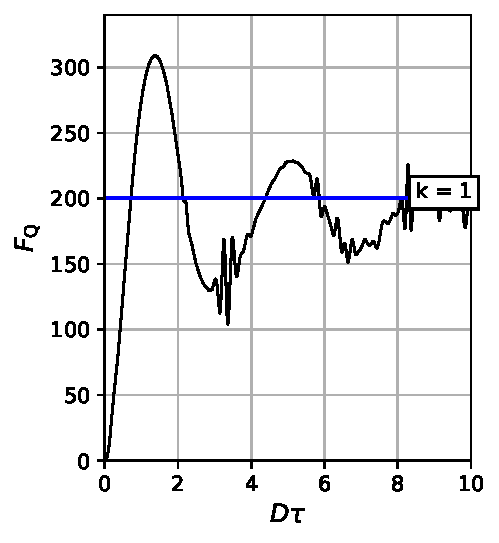
\includegraphics[width=\textwidth]{m2_t_b01.pdf}
    \caption{
      ${T=2.4\cdot10^{-1}}$~K $(b=0.1)$.
      Парная запутанности выше горизонтальной линии.
      %The inequality~(\ref{eq:fisher_criteria}) yields the region of pair entanglement $(k+1=2)$.
      %The region is above the horizontal line.
    }
    \label{fig:m2_t_b01}
  \end{subfigure}
  \hfill
  \begin{subfigure}[t]{0.4\textwidth}
    %\centering
    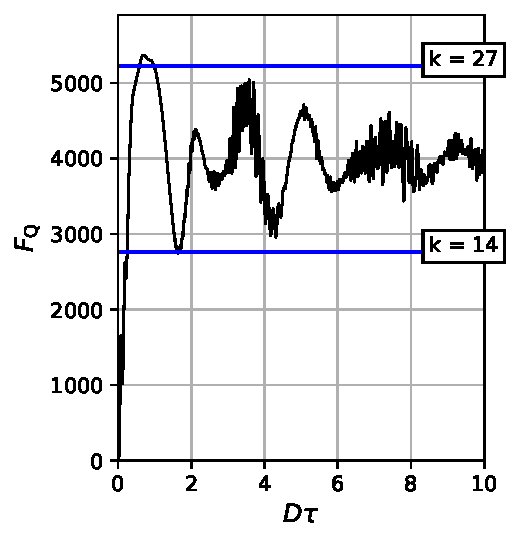
\includegraphics[width=\textwidth]{m2_t_b05.pdf}
    \caption{
      ${T=4.8\cdot10^{-2}}$~K $(b=0.5)$.
      Область многоспиновой запутанности представляет собой полосу, ограниченную горизонтальными линиями с $k=14$ и $k=27$.
      }
    \label{fig:m2_t_b05}
  \end{subfigure}
  \hfill
  \begin{subfigure}[t]{0.4\textwidth}
    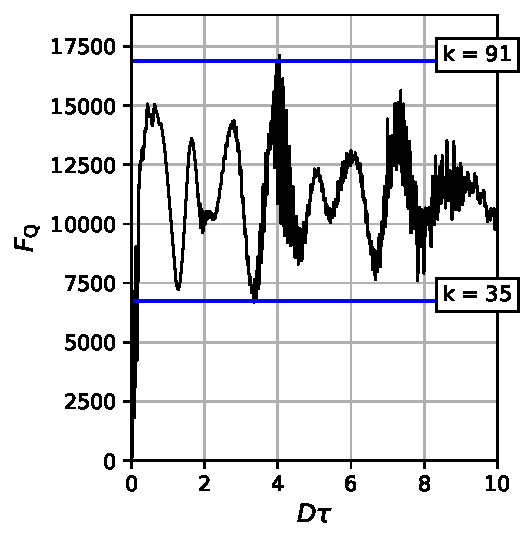
\includegraphics[width=\textwidth]{m2_t_b1.pdf}
    \caption{
      ${T=2.4\cdot10^{-2}}$~K $(b=1)$.
    }
    \label{fig:m2_t_b1}
  \end{subfigure}
  \hfill
  \begin{subfigure}[t]{0.4\textwidth}
    %\centering
    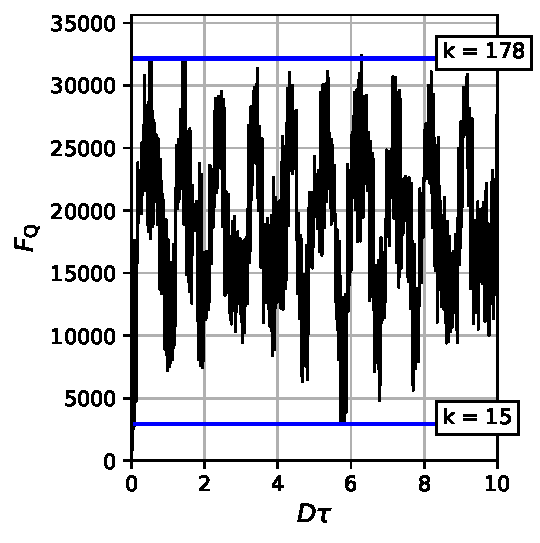
\includegraphics[width=\textwidth]{m2_t_b3_5.pdf}
    \caption{
      ${T=6.856\cdot10^{-3}}$~K $(b=3.5)$.
      Почти все спины (до $179$ из $201$) могут быть частью запутанного кластера.
    }
  \label{fig:m2_t_b3.5}
  \end{subfigure}
  \caption{
    Зависимость нижней границы квантовой информации Фишера $F_Q = 2M_2(\tau)$ от безразмерного времени $D\tau$.
    Горизонтальные линии ограничивают полосу с многоспиновой запутанностью.
  }
\end{figure}

Интенсивности приведенных МК когерентностей  ЯМР определяются уравнениями ~(\ref{eq:j_lt},~\ref{eq:j_lt_norm}) как при высоких ($b < 1$), так и при низких ($b > 1$) температурах.
Нижняя граница квантовой информации Фишера может быть посчитана из выражений
~(\ref{eq:j_lt}),~(\ref{eq:j_lt_norm}),~(\ref{eq:fisher-low-bound})~и~(\ref{eq:m2-via-coherences}).

Значение параметра $b = 0.1$, соответствует температуре ${T= 2.4\cdot 10^{-1}}$~K при Ларморовской частоте $\omega_0 = 2\pi\cdot 500\cdot10^6$ с$^{-1}$ (рис.~\ref{fig:m2_t_b01}).
Неравенство~(\ref{eq:entanglement-criteria}) может быть выполнено только при $k=1$ (горизонтальная линия на рис.~\ref{fig:m2_t_b01}).
Это означает, что парная запутанность возможна в высокотемпературном случае \cite{Feldman2012}.

При температуре ${4.8\cdot10^{-2}}$~K $(b=0.5)$ видна полоса (рис.~\ref{fig:m2_t_b05}), в которой неравенство~(\ref{eq:entanglement-criteria}) может быть удовлетворено, когда $14 \leq k \leq 27$.

Таким образом, при температуре ${4.8\cdot10^{-2}}$~K в спиновых кластерах, состоящих из 15-28 спинов, существует многоспиновая запутанность. При понижении температуры ширина полосы, где существует многоспиновая запутанность, увеличивается. При температуре ${2.4\cdot10^{-2}}$~K $(b=1)$ (рис.~\ref{fig:m2_t_b1}) в такой полосе число запутанных спинов может составлять от 36 до 92.

Наконец, при температуре ${T= 6.856\cdot10^{-3}}$~K $(b=3.5)$ (рис.~\ref{fig:m2_t_b3.5}), почти все спины (до 179 из 201) запутаны. Запутанность существует в течение всего процесса эволюции, за исключением короткого начального периода времени.

На рис.\ref{fig:k_b} показано, что количество запутанных спинов увеличивается при понижении температуры.


Таким образом, предложенная модель нанополости, заполненной спин-несущими атомами (молекулами), позволяет исследовать многоспиновую запутанность и ее зависимость от температуры.

\begin{figure}[H]
  \centering
  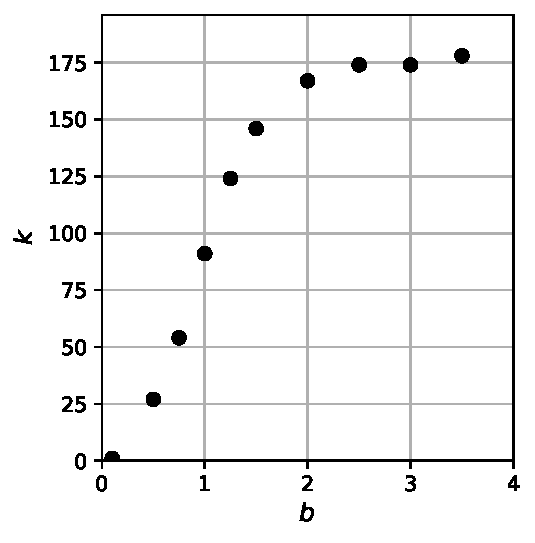
\includegraphics{k_b.pdf}
  \caption{Зависимость числа запутанных спинов от параметра  $b = \frac{\hbar\omega_0}{kT} $.}
  \label{fig:k_b}
\end{figure}



\section{Дипольное упорядоченное состояние}
\label{sec:1}

В предыдущем разделе~\ref{sec:nanopora-thermodynamic-equilibrium} была исследована многоспиновая запутанность для несферической нанопоры~\cite{Doronin2019},
заполненной газом  спин-несущих молекул в сильном внешнем магнитном поле~\cite{Baugh2001,Doronin2009}.
Термодинамическое равновесное начальное состояние системы определялось односпиновым зеемановским взаимодействием с внешним магнитным полем~\cite{Doronin2007a}.
Однако  многоспиновую запутанность можно  исследовать,
когда та же самая система первоначально подготовлена в дипольном упорядоченном состоянии~\cite{Goldman1970}.
Главной мотивацией выбора такого начального состояния является результат полученный в работе~\cite{Doronin2011}.
В частности было показано, что в МК~эксперименте~ЯМР~с дипольным упорядоченным начальным состоянием МК~когерентности~ЯМР~возникают быстрее,
чем в МК~эксперименте~ЯМР~с начальным термодинамическим равновесным состоянием в сильном внешнем магнитном поле.
Данное обстоятельство является важным для исследования многоспиновой запутанности,
поскольку при этом используется второй момент распределения МК~когерентностей~ЯМР.

В общем случае в начальный момент система находится в термодинамическом равновесии с матрицей плотности
%
\begin{equation}\label{eq:4}
    \rho(0) = \rho_\mathrm{eq} = \dfrac{1}{Z}
    e^{
      \frac{\hslash \omega_{0}}{k} \alpha_\mathrm{z} I_\mathrm{z}
      + \frac{\hslash }{k} \beta_\mathrm{d} H_\mathrm{dz}
    },
\end{equation}
%
где
$Z = \mathrm{Tr} \left\{ e^{\frac{\hslash \omega_{0}}{k} \alpha_\mathrm{z} I_\mathrm{z} + \frac{\hslash }{k} \beta_\mathrm{d} H_\mathrm{dz}} \right\}$ - статистическая сумма,
$\hslash$ и $k$ - константы Планка и Больцмана,
$\omega_{0}$ - частота Лармора,
$I_\mathrm{z}$ -  оператор проекции полного углового спинового момента  на ось~$z$,
который направлен вдоль сильного внешнего магнитного поля,
$H_\mathrm{dz}$ - секулярная часть гамильтониана ДДВ в сильном внешнем магнитном поле
и $\alpha_\mathrm{z}$, $\beta_\mathrm{d}$ - обратные зеемановская и дипольная температуры.
%
Используя  метод адиабатического размагничивания во вращающейся системе координат (ВСК)~\cite{Goldman1970, Slichter1961},
либо двухимпульную последовательность Брокаерта-Джинира~(см. подраздел~\ref{seq:jeener-sequence})
можно получить систему в состоянии термодинамического равновесия с матрицей плотности
%
\begin{equation}\label{eq:5a}
  \rho_i = \frac{1}{Z_i} e^\frac{\hslash\beta_\mathrm{d} \hdz}{k},
  %approx \frac{1}{Z_i}(1 + \frac{\hslash\beta_\mathrm{d}}{k} H_\mathrm{dz}),
\end{equation}
%
где статистическая сумма
%
\begin{equation}\label{eq:6}
  Z_i = \mathrm{Tr} \left\{ e^\frac{\hslash\beta_\mathrm{d} \hdz}{k} \right\} \approx 2^{N}.
\end{equation}
%
Магнитное упорядочение~\cite{Abragam1982} выходит за рамки данного раздела,
поэтому будет рассмотрен промежуточный температурный случай,
когда зеемановская температура является низкой $({\frac{\hslash \omega_{0}}{k} \alpha_\mathrm{z}}\gg 1)$,
а дипольная - высокой $\left( \frac{\hslash{D}}{k}\beta_\mathrm{d} \ll 1\right)$.
Тогда выражение~(\ref{eq:5a}) матрицы плотности~$\rho_i$ может быть разложено в ряд по $b$:
%
\begin{equation}\label{eq:5}
  \rho_i \approx \frac{1}{Z_i}(1 + \frac{\hslash\beta_\mathrm{d}}{k} H_\mathrm{dz}),
\end{equation}
%
Гамильтониан $H_{dz}$ частично усредняется быстрой молекулярной диффузией в нанопоре,
и может быть записан~\cite{Feldman2004,Doronin2011} как
%
\begin{equation}
  \label{eq:7}
  H_\mathrm{dz} = \dfrac{D}{2} (3 I^{2}_{z} - I^{2}) , % ?
\end{equation}
%
где $I^{2}$ - квадрат углового спинового  момента.

После периодов подготовки, эволюции и смешивания в МК~эксперименте~ЯМР~(см. раздел~\ref{sec:mq-nrm-experiment})
сигнал усредненный по равновесной матрице плотности $\rho_i$
имеет вид~(см. раздел~\ref{sec:reduced-mq-coherences})
%
\begin{equation}\label{eq:signal-do}
  \begin{split}
    G_\mathrm{DO}(\tau,\phi)
    & = \mathrm{Tr}\left\{
      e^{i H_\mathrm{MQ} \tau} e^{i\phi I_\mathrm{z}} e^{-i H_\mathrm{MQ}\tau}
      \rho_i
      e^{i H_\mathrm{MQ} \tau} e^{-i \phi I_\mathrm{z}} e^{-i H_\mathrm{MQ} \tau}
      \rho_i
    \right\} \\
    & = \mathrm{Tr} \left\{
    e^{i \phi I_\mathrm{z}}
    \rho_\mathrm{DO}(\tau)
    e^{-i \phi I_\mathrm{z}}
    \rho_\mathrm{DO}(\tau)
    \right\},
  \end{split}
\end{equation}
%
где
%
\begin{equation}
  \label{eq:9}
  \rho_\mathrm{DO}(\tau)
  = e^{-i H_\mathrm{MQ} \tau }
  \rho_i
  e^{i H_\mathrm{MQ} \tau}
\end{equation}
%
является решением уравнения~(\ref{eq:3}) при начальном условии~(\ref{eq:5}).
Выражение~\ref{eq:signal-d} сигнала  $G_\mathrm{DO}G_\mathrm{HT}(\tau,\phi)$,
является неупорядоченные по времени коррелятором~(см. раздел~\ref{sec:reduced-mq-coherences}),
следовательно, второй момент коррелятора $G_\mathrm{DO}(\tau,\phi)$ определяет
нижнюю границу квантовой информации Фишера~(см. раздел~\ref{sec:reduced-mq-coherences}).
Нормированные интенсивности $J_{n}(\tau)$ $(n=0, \pm 2, \pm 4, \cdots)$ МК~когерентностей~ЯМР
имеют вид
%
\begin{equation}\label{eq:13}
  J_{n}(\tau) = \dfrac{\mathrm{Tr} \left\{
  \rho_{n}(\tau) \rho_{-n}(\tau)
  \right\}}
  {\mathrm{Tr} \left\{\rho^2_{i} \right\}}
\end{equation}


Матрица плотности~$\rho_i$ и гамильтониан $H_\mathrm{MQ}$,
имеют блочную структуру в мультипликативном базисе~(см. раздел~\ref{sec:model-equivalent-spins}).
Следовательно, как и в предыдущем разделе~\ref{sec:nanopora-thermodynamic-equilibrium},
вычисление выражения~\ref{eq:13} интенсивности приведенной МК когерентности ЯМР сводится
к вычислению отдельных вкладов
для каждого значения полного спинового углового момента $S$~(см. выражение~\ref{eq:coherence_k}).
Используя этот метод, можно исследовать МК~динамику~ЯМР~в системах, состоящих из сотен спинов.


% \subsection{Двухимпульсный эксперимент Брокаерта-Джинера при низкой зеемановской температуре и высокой дипольной температуре.}
\subsection{Двухимпульсный эксперимент Брокаерта-Джинера.}
\label{seq:jeener-sequence}

Оригинальный двухимпульсный эксперимент Брокаерта-Джинира~\cite{Jeener1967} был разработан  для высокотемпературного случая,
однако ниже будет показано,
что двухимпульсная последовательность Брокаерта-Джинера~\cite{Goldman1970,Jeener1967}
позволяет получить дипольное упорядоченное состояние
даже при низкой зеемановской температуре.

Изначально система находится в состоянии термодинамического равновесия в сильном внешнем магнитном поле с матрицей плотности
%
\begin{equation}
  \label{eq:a1}
  \sigma_{i} = \dfrac{e^{\beta_\mathrm{L} \omega_{0} I_\mathrm{z}}}{Z_{i}} ,
  \quad
  Z_{i} = \mathrm{Tr}\left\{e^{\beta_\mathrm{L} \omega_{0} I_\mathrm{z}} \right\}
\end{equation}
%
После первого резонансного $x$-импульса получаем
%
\begin{equation}
  \label{eq:a2}
  \sigma'(0) = e^{ i \frac \pi 2 I_\mathrm{x}}
  \sigma_{i}
  e^{-i \frac \pi 2 I_\mathrm{x}}
  = \dfrac{e^{\beta_\mathrm{L} \omega_{0} I_\mathrm{y}}}{Z_{i}} .
\end{equation}
%
Затем система свободно эволюционирует в течение времени $\tau$,
и после этого подается второй резонансный $y$-импульс, который поворачивает спины на угол $\theta$ вокруг оси-$y$ ВСК.
В результате получаем, что
\begin{equation}
  \label{eq:a3}
  \sigma'(\tau)
  = \dfrac{
   e^{-i \theta I_\mathrm{y}} e^{-i H_\mathrm{dz} \tau}
   e^{\beta_\mathrm{L} \omega_{0} I_\mathrm{y}}
   e^{i H_\mathrm{dz} \tau} e^{i \theta I_\mathrm{y}}
  }{Z_{i}}.
\end{equation}
%
По истечении времени $T_2$ ($T_2$ - время спиновой релаксации \cite{Goldman1970}) система достигает состояния термодинамического равновесия
\begin{equation}
  \label{eq:a4}
  \sigma_{f}
  = \dfrac{ e^{\alpha \omega_{0} I_\mathrm{z} + \beta H_\mathrm{dz}} }{Z_f},
\end{equation}
%
где $\alpha$ и $\beta$ - обратные зеемановская и дипольная температуры.
Очевидно, что система имеет единственное  равновесное состояние, а
 температуры $\alpha$ и $\beta$ в равновесном состоянии находятся из
законов сохранения:

\begin{align}
  \label{eq:a5}
  \mathrm{Tr} \left\{ I_\mathrm{z} \sigma'(\tau) \right\}
  & = \mathrm{Tr} \left\{ I_\mathrm{z} \sigma_{f}(\tau) \right\}
  \\
  \label{eq:a6}
  \mathrm{Tr} \left\{ H_\mathrm{dz} \sigma'(\tau) \right\}
  & = \mathrm{Tr} \left\{ H_\mathrm{dz} \sigma_{f}(\tau) \right\}
\end{align}
%
Можно переписать $\mathrm{Tr} \left\{ I_\mathrm{z} \sigma'(\tau) \right\}$ как
%
\begin{multline}
  \label{eq:a7}
  \tr{I_\mathrm{z} \sigma'(\tau)}
  = \dfrac{1}{Z_{i}} \tr{
    e^{i \theta \sy} \sz e^{-i \theta \sy}
    e^{-i \hdz \tau} e^{\beta_\mathrm{L} \omega_{0} \sy} e^{i \hdz \tau}
  }
  \\
  = \dfrac{1}{Z_i} \tr{
    \left( \cos(\theta) \sz - \sin(\theta) \sx \right)
    e^{-i \hdz \tau} e^{\beta_\mathrm{L} \omega_{0} \sy} e^{i \hdz \tau}
  }
  \\
  = \dfrac{1}{Z_i} \tr{
    e^{-i \pi \sy}
    \left( \cos(\theta) \sz - \sin(\theta) \sx \right)
    e^{-i \hdz \tau} e^{\beta_\mathrm{L} \omega_{0} \sy} e^{i \hdz \tau}
    e^{i \pi \sy}
  }
  \\
  = - \dfrac{1}{Z_i} \tr{
    \left( \cos(\theta) \sz - \sin(\theta) \sx \right)
    e^{-i \hdz \tau} e^{\beta_\mathrm{L} \omega_{0} \sy} e^{i \hdz \tau}
  } = 0
\end{multline}
%
В~(\ref{eq:a7}) было учтено, что $\left[ e^{-i \pi \sy}, \hdz \right] = 0$.
Поскольку мы рассматриваем случай высокой дипольной температуры, можно переписать уравнение~(\ref{eq:a5}) как
\begin{equation}
  \label{eq:a8}
  0 = \dfrac{1}{Z_f} \tr{ \sz e^{\alpha \omega_{0} \sz}}
  + \dfrac{\beta}{Z_f} \tr{\sz e^{\alpha \omega_{0} \sz} \hdz}.
\end{equation}
%
Заметим, что $\tr{\sz} = \tr{\sz\hdz} = 0$.
В таком случае $\alpha = 0$ удовлетворяет уравнению~(\ref{eq:5}).
Таким образом, в рассматриваемом случае мы получаем дипольное упорядоченное состояние.


% \subsection{Аналитическое решение для МК~динамики~ЯМР~трехспиновой системы в нанопоре в дипольном упорядоченном состоянии}
\subsection{Аналитическое решение для трехспиновой системы}
\label{sec:3}

\begin{figure}[H]
  \centering
 	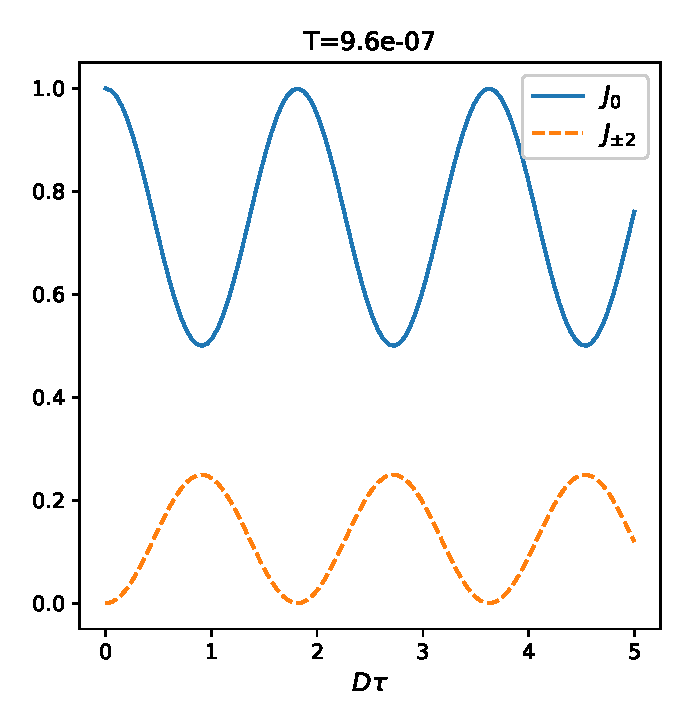
\includegraphics[width=0.5\linewidth]{coherences_n3_beta5.eps}
	\caption{
	  Интенсивности МК~когерентностей~ЯМР~$J_{n}$ ($n=0, 2$) в нанопоре с $N=3$.
      Здесь предполагается, что $\omega_{0} = 2\pi \cdot 500 \cdot 10^{6}$~s$^{-1}$ и $D = 2\pi \cdot 10^{4}$~s$^{-1}$.
	}
	\label{fig:1}
\end{figure}

В этом разделе будет получено точное решение МК~динамики~ЯМР~трехспиновой системы в дипольном упорядоченном состоянии в нанопоре.
Решение будет получена в общем виде, без использования высокотемпературного приближения~\cite{Goldman1970}.
Данная задача аналогична задаче, рассмотренной в разделе~\ref{sec:nanopora-thermodynamic-equilibrium}
для начального термодинамического равновесия в сильном внешнем магнитном поле.

Гамильтониан $H_{MQ}$ уравнения~(\ref{eq:hmq}) состоит из двух блоков для двух возможных значений углового момента спина $(I^2 = S(S+1), \quad S=3/2,1/2)$.
Эти блоки и соответствующие им собственные значения и собственные состояния приведены
в разделе~\ref{sec:sec:nanopora-thermodynamic-equilibrium-exact_sol}.
Матрица плотности системы также состоит из двух блоков $\rho^{3/2}(\tau)$, $\rho^{1/2}(\tau)$, и
%
\begin{equation}
  \label{eq:15}
  \rho^{3/2}(0) = \dfrac 1 Z
  \begin{pmatrix}
    e^{\frac{3b}{2}} & 0 & 0 & 0
    \\
    0 & e^{\frac{-3b}{2}} & 0 & 0
    \\
    0 & 0 & e^{\frac{-3b}{2}} & 0
    \\
    0 & 0 & 0 & e^{\frac{3b}{2}}
  \end{pmatrix},
  \quad
  \rho^{1/2}(0) = \dfrac 1 Z
  \begin{pmatrix}
    	1 & 0
    \\
    0 & 1
  \end{pmatrix}
\end{equation}
%
где $b = \dfrac{\hslash D}{k\mathrm{T}}$ и $T$ --- температура.
Простыми вычислениями можно получить матрицы плотности $\rho^{3/2}(\tau)$ и $\rho^{1/2}(\tau)$,
которые позволяют получить выражение для интенсивности МК~когерентностей~ЯМР.

В рассматриваемых системах появляются только МК~когерентности~ЯМР нулевого и плюс/минус второго порядков.
Интенсивности этих когерентностей равны
%
\begin{equation}
  \begin{split}
    \label{eq:16}
    J_0(\tau) & = 1
    - \dfrac 1 2 \tanh^2\left( \dfrac{3b}{2} \right)
      \sin^2 \left( \sqrt{3} Dt \right),
    \\
    J_{\pm2}(\tau) & = \dfrac{1}{4}
      \tanh^2 \left( \dfrac{3b}{2} \right)
      \sin^2 \left( \sqrt{3} Dt \right)
  \end{split}
\end{equation}
%
Сумма интенсивностей МК когерентностей согласно~(\ref{eq:16}) равна единице в соответствии с уравнением~(\ref{eq:14}).
Зависимости рассчитанных интенсивностей $J_{n}(\tau)$ $(n=0,2)$ от времени эволюции показаны на рисунке~(\ref{fig:1}).

% \subsection{Численный анализ многоспиновой запутанности при различных температурах и различном числе спинов в системе}
\subsection{Температурная зависимость многочастичной запутанности}
\label{sec:5}

В этом разделе приведены результаты полуаналитической симуляции МК эксперимента ЯМР
для модели спин-несущих молекул (атомов) в нанопоре в дипольном упорядоченном состоянии.
Будет рассмотрена зависимость нижней границы квантовой информации Фишера от времени и температуры.
А также получены оценки количества запутанных частиц в системе.
В расчетах предполагается, что $\omega_{0} = 2\pi \cdot 500 \cdot 10^{6}$~s$^{-1}$ и $D = 2\pi \cdot 10^{4}$~s$^{-1}$.

\begin{figure}[H]
 	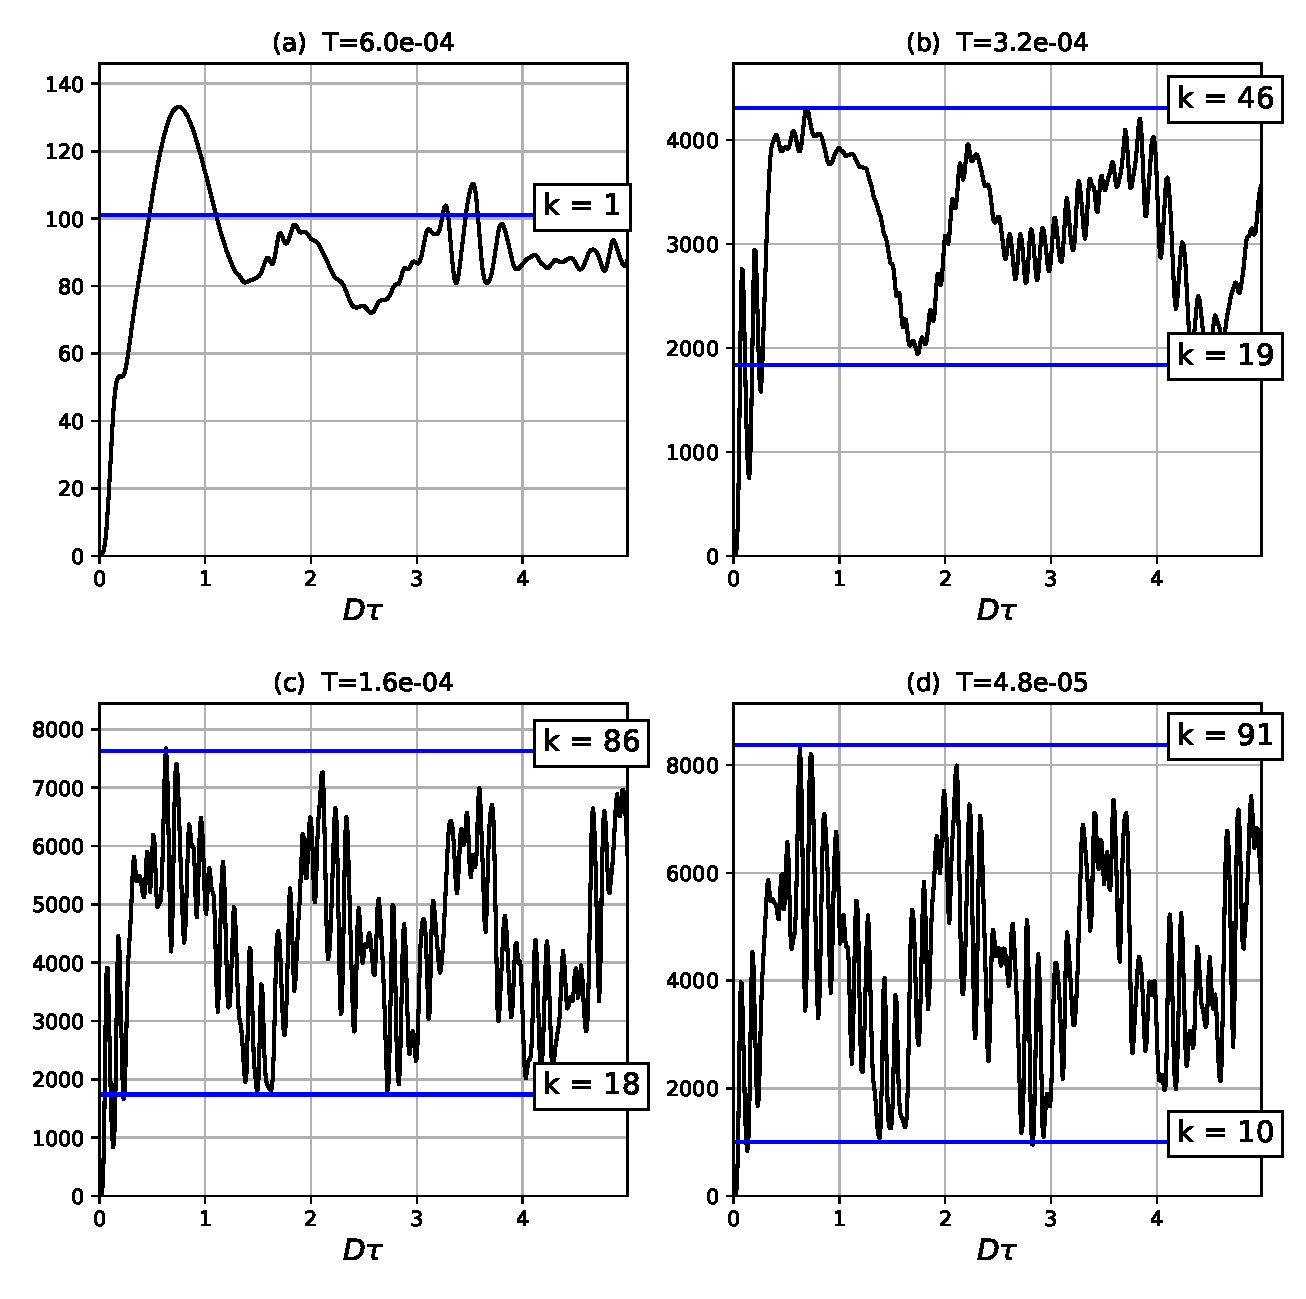
\includegraphics[width=0.95\linewidth]{fisher_low_bound_n101.eps}
	\caption{
	  Зависимость нижней границы  квантовой информации Фишера $F_\mathrm{Q} = 2 M_{2}$
	  от безразмерного времени $D\tau$ при $N=101$.
	  a) $T=6\cdot10^{-4}$~K, неравенство~(\ref{eq:20}) определяет область парной запутанности  (k+1=2), эта область выше горизонтальной линии;
	  b) $T=3.2\cdot10^{-4}$~K, область многоспиновой запутанности представляет собой полосу, ограниченную горизонтальными линиями с~$k=19$~и~$k=46$;
	  c) $T = 1.6\cdot10^{_4}$~K, горизонтальные линии ($k=18$ и $k=86$) ограничивают полосу с многоспиновой запутанностью;
	  d) при $T=4.8\cdot10^{-5}$~K возникают запутанные кластеры с $11-92$ спинами.
	}
	\label{fig:2}
\end{figure}


Рассматриваемая модель спин-несущих молекул (атомов) в нанопоре в дипольном упорядоченном состоянии
расширяет возможности исследования многоспиновой запутанности по сравнению с родственной моделью~(см. раздел~\ref{sec:nanopora-thermodynamic-equilibrium}),
в которой система изначально находилась в термодинамическом равновесии в сильном внешнем магнитном поле.
Модель из раздела~\ref{sec:nanopora-thermodynamic-equilibrium}) неприменима для исследования эволюции системы во времени,
потому что распределение МК~когерентностей~ЯМР~быстро становится стационарным~\cite{Doronin2009}.
Также многоспиновая запутанность изменяется с температурой в очень узком температурном интервале.
Например, все спины запутаны в системе, состоящей из 201 спина уже при температуре $T=6.856\cdot10^{-3}$~K~\cite{Doronin2019}.

Зависимость нижней границы квантовой информации Фишера от времени в системе, состоящей из 101 спина, представлена на Рис.~(\ref{fig:2}) при различных температурах.
Из Рис.~(\ref{fig:2}a) видно, что при температуре $T=6\cdot10^{-4}$~K существует только парная запутанность.
При температуре $T=3.2\cdot10^{-4}$ на Рис.~(\ref{fig:2}b) появляется полоса, в которой неравенство~(\ref{eq:entanglement-criteria}) может быть выполнено, когда $19 \leq k \leq 46$.
Таким образом, существует многоспиновая запутанность в спиновых кластерах, состоящих из 20-47 спинов, при температуре $3.2\cdot10^{-4}$~K.
Когда температура понижается, ширина полосы, в которой существует многоспиновая запутанность, увеличивается.
При температуре $T=1.6\cdot10^{-4}$~K (Рис.~(\ref{fig:2}c)) появляются кластеры из 19-87 запутанных спинов, а при температуре $T=4.8\cdot10^{-5}$~K (Рис.~(\ref{fig:2}d)), наблюдаются 11-92 запутанных спина.

\begin{figure}
 	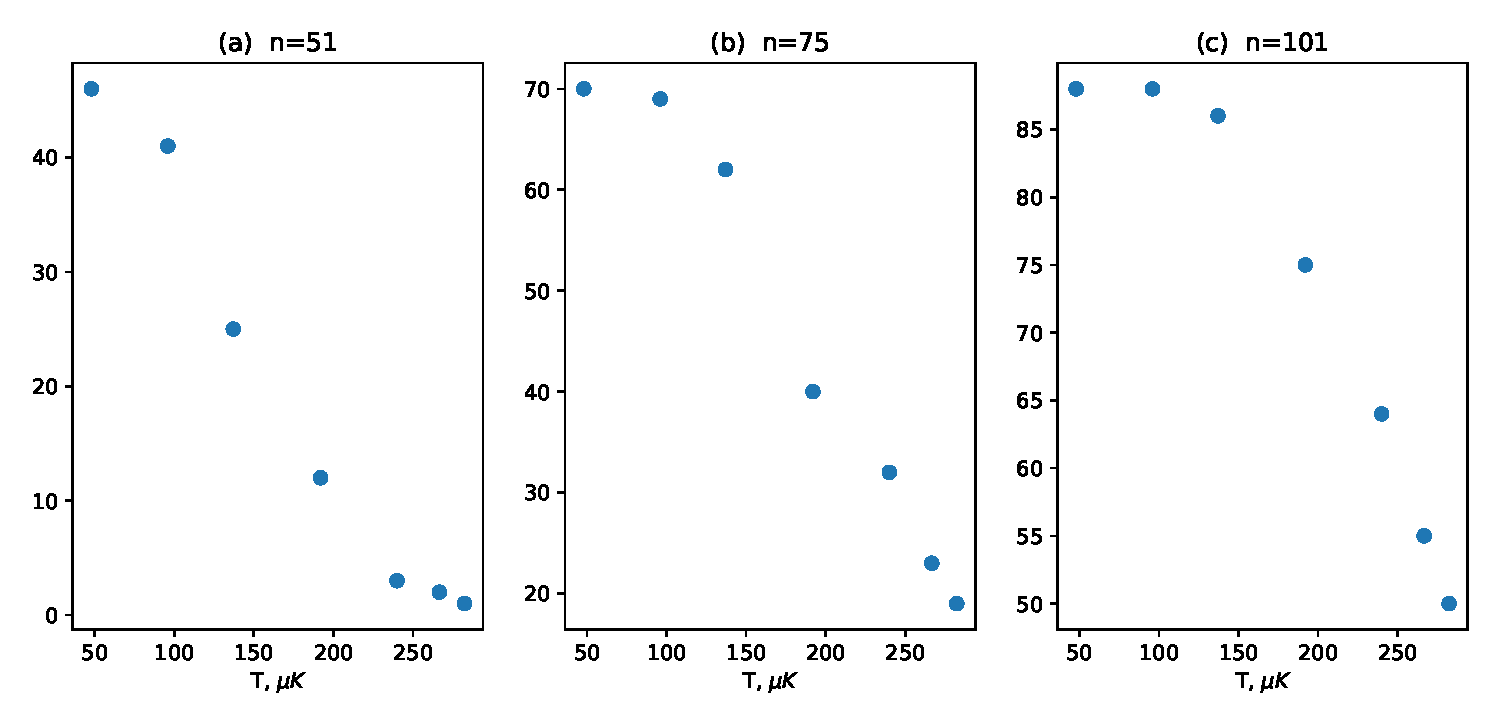
\includegraphics[width=0.95\linewidth]{entangled_spins_by_n.eps}
	\caption{
	  Зависимость максимального количества запутанных спинов,
	  усредненного по времени эволюции $(0 \leq D\tau \leq 3)$,
	  от температуры при  a) $N=51$; b) $N=75$; c) $N=101$.
	}
	\label{fig:3}
\end{figure}

Зависимость максимального числа запутанных спинов за время эволюции $({0}\leq \mathrm{D}\tau\leq{3})$ от температуры при разных числах спинов в нанопоре представлена на Рис.~(\ref{fig:3}).
Максимальное количество запутанных спинов уменьшается при повышении температуры.
Максимальное количество запутанных спинов увеличивается, когда увеличивается число спинов в нанопоре, потому что система в нанопоре становится плотнее.

\section{Выводы}
\label{sec:conslusions}
% We investigated many-particle entanglement in MQ NMR spectroscopy using a nanocavity filled with spin-carrying atoms (molecules).
% We developed a theory of MQ NMR in a nanocavity at low temperatures.
% The theory is based on the idea that  molecular diffusion is substantially faster than the time of the spin flip-flop processes.
% As a result, the problem is reduced to a system of equivalent spins [23, 25], which can be analyzed in the basis of the common eigenstates of the total spin angular momentum and its projection on the external magnetic field.
% Since there is a connection between the second moment (dispersion) of the distribution of the MQ NMR intensities and many-spin entanglement [17], we extracted information about many-spin entanglement from the MQ NMR spectrum. The temperature dependence of many-spin entanglement was also investigated.
% \par
% The main lesson consists in significant growth of many-particle entanglement at low temperatures.
% All or almost all spins are entangled at the dimensionless temperature $\frac{1}{b}$ of the order of 1.
% This suggests that $k$-entangled states with large $k$ emerge in a typical MQ NMR system at low temperatures.
% This is particularly interesting given the absence of entanglement in the initial state. We expect such behavior to be typical for MQ NMR.
% \par
% We can conclude that MQ NMR spectroscopy is an effective method for the investigation of many-spin entanglement and the spreading of MQ correlations inside many-spin systems. It can be used for experimental investigations of quantum information processing in solids (note a related study of decoherence in liquids \cite{HOU2017863}).
% \par

В этой главе была исследована многочастичная запутанность в МК спектроскопии ЯМР в нанопоре, заполненной сотнями спин-несущими частицами.
Для этого была разработана МК теория ЯМР в нанопоре при низких температурах.
Было рассмотрено два начальных состояния системы:
термодинамически равновесное
и дипольное упорядоченное.
В обоих случах впервые удалось исследовать температурную зависимость многочастичной запутанности.
Все или почти все спины запутаны при безразмерной температуре $\frac{1}{b}$ порядка 1.
Это говорит о том, что $k$-запутанные состояния с большим $k$ возникают в типичной системе МК ЯМР при низких температурах.
Это особенно интересно, учитывая отсутствие запутанности в начальном состоянии.
Можно заключить, что такое поведение типично для МК ЯМР.
Так же была исследована зависимость многоспиновой запутанности
от количества спинов в нанопоре.
Показано, что с ростом количества спинов в нанопоре,
скорость возникновения запутанных кластеров при понижении температуры увеличивается.

Результаты этого раздела наглядно демонстрируют
универсальность разработанного в этой диссертации метода исследования многочастичной запутанности.
